% Options for packages loaded elsewhere
\PassOptionsToPackage{unicode}{hyperref}
\PassOptionsToPackage{hyphens}{url}
%
\documentclass[
]{book}
\usepackage{amsmath,amssymb}
\usepackage{lmodern}
\usepackage{ifxetex,ifluatex}
\ifnum 0\ifxetex 1\fi\ifluatex 1\fi=0 % if pdftex
  \usepackage[T1]{fontenc}
  \usepackage[utf8]{inputenc}
  \usepackage{textcomp} % provide euro and other symbols
\else % if luatex or xetex
  \usepackage{unicode-math}
  \defaultfontfeatures{Scale=MatchLowercase}
  \defaultfontfeatures[\rmfamily]{Ligatures=TeX,Scale=1}
\fi
% Use upquote if available, for straight quotes in verbatim environments
\IfFileExists{upquote.sty}{\usepackage{upquote}}{}
\IfFileExists{microtype.sty}{% use microtype if available
  \usepackage[]{microtype}
  \UseMicrotypeSet[protrusion]{basicmath} % disable protrusion for tt fonts
}{}
\makeatletter
\@ifundefined{KOMAClassName}{% if non-KOMA class
  \IfFileExists{parskip.sty}{%
    \usepackage{parskip}
  }{% else
    \setlength{\parindent}{0pt}
    \setlength{\parskip}{6pt plus 2pt minus 1pt}}
}{% if KOMA class
  \KOMAoptions{parskip=half}}
\makeatother
\usepackage{xcolor}
\IfFileExists{xurl.sty}{\usepackage{xurl}}{} % add URL line breaks if available
\IfFileExists{bookmark.sty}{\usepackage{bookmark}}{\usepackage{hyperref}}
\hypersetup{
  pdftitle={Elektra: Forecasting DEMO},
  hidelinks,
  pdfcreator={LaTeX via pandoc}}
\urlstyle{same} % disable monospaced font for URLs
\usepackage{longtable,booktabs,array}
\usepackage{calc} % for calculating minipage widths
% Correct order of tables after \paragraph or \subparagraph
\usepackage{etoolbox}
\makeatletter
\patchcmd\longtable{\par}{\if@noskipsec\mbox{}\fi\par}{}{}
\makeatother
% Allow footnotes in longtable head/foot
\IfFileExists{footnotehyper.sty}{\usepackage{footnotehyper}}{\usepackage{footnote}}
\makesavenoteenv{longtable}
\usepackage{graphicx}
\makeatletter
\def\maxwidth{\ifdim\Gin@nat@width>\linewidth\linewidth\else\Gin@nat@width\fi}
\def\maxheight{\ifdim\Gin@nat@height>\textheight\textheight\else\Gin@nat@height\fi}
\makeatother
% Scale images if necessary, so that they will not overflow the page
% margins by default, and it is still possible to overwrite the defaults
% using explicit options in \includegraphics[width, height, ...]{}
\setkeys{Gin}{width=\maxwidth,height=\maxheight,keepaspectratio}
% Set default figure placement to htbp
\makeatletter
\def\fps@figure{htbp}
\makeatother
\setlength{\emergencystretch}{3em} % prevent overfull lines
\providecommand{\tightlist}{%
  \setlength{\itemsep}{0pt}\setlength{\parskip}{0pt}}
\setcounter{secnumdepth}{5}
\usepackage{booktabs}
\renewcommand{\contentsname}{Contenido} \usepackage{caption} \captionsetup[figure]{name=Figura} \setlength\headheight{12.80502pt} \usepackage{fancyhdr} \pagestyle{fancy} \fancyhead[LE,RO]{\textsl{\rightmark}} \fancyhead[LO,RE]{\textsl{\leftmark}} \usepackage{float}
\ifluatex
  \usepackage{selnolig}  % disable illegal ligatures
\fi
\usepackage[]{natbib}
\bibliographystyle{apalike}

\title{Elektra: Forecasting DEMO}
\usepackage{etoolbox}
\makeatletter
\providecommand{\subtitle}[1]{% add subtitle to \maketitle
  \apptocmd{\@title}{\par {\large #1 \par}}{}{}
}
\makeatother
\subtitle{Análisis Exploratorio de Datos}
\author{}
\date{\vspace{-2.5em}}

\begin{document}
\maketitle

{
\setcounter{tocdepth}{1}
\tableofcontents
}
\hypertarget{introducciuxf3n}{%
\chapter*{Introducción}\label{introducciuxf3n}}
\addcontentsline{toc}{chapter}{Introducción}

Este documento presenta los hallazgos iniciales en los datos usados para realizar el \textbf{DEMO} de pronósticos de ventas de \emph{Elektra} a través de la plataforma de e-commerce. La documentación es creada a partir de los archivos entregados por parte de \emph{DDI}. En este análisis se realiza una inspección minuciosa a cada uno de los atributos y eventos asociados a las actividades de marketing y ventas diarias que ocurren a través de la plataforma de Elektra Gt.

\begin{center}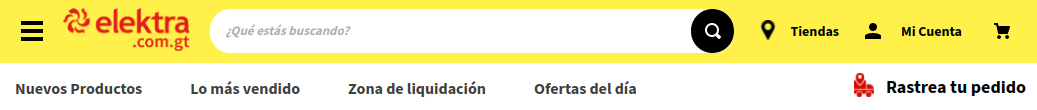
\includegraphics[width=650pt,height=75pt]{img/00-intro/ecommerce} \end{center}

\begin{center}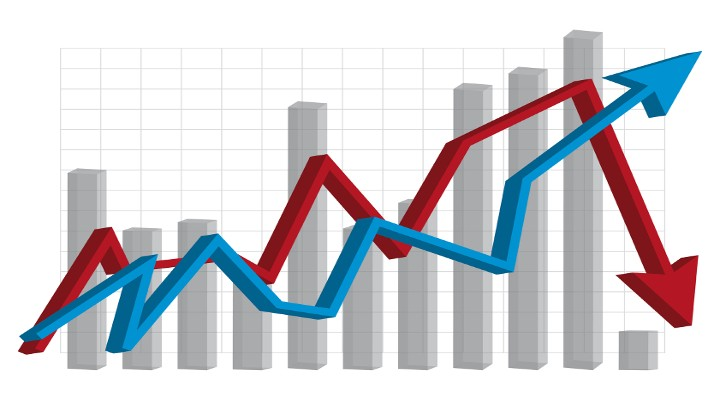
\includegraphics[width=700pt,height=250pt]{img/00-intro/forecasting} \end{center}

\hypertarget{objetivo}{%
\section*{Objetivo}\label{objetivo}}
\addcontentsline{toc}{section}{Objetivo}

Los insumos entregados por parte de \textbf{DDI} serán usados para desarrollar las actividades que se han planteado en el objetivo del proyecto, las cuales se enlistan a continuación:

\begin{enumerate}
\def\labelenumi{\arabic{enumi}.}
\item
  \textbf{Predicción:} predecir las ventas (en un rango) de e-commerce de Elektra, a total plataforma, diarias para una semana (de lunes a domingo), con cuatro días de anticipación (el jueves previo al primer día de predicción).
\item
  \textbf{Data Storytelling:} producir insights sobre las ventas y las variables que afectan a éstas mediante gráficas comparativas multivariadas.
\item
  \textbf{Machine Learning:} Automatizar el pipeline de ingesta y procesamiento de datos y de ejecución del modelo de predicción de ventas sobre la infraestructura (Data Warehouse) de \emph{DDI}.
\end{enumerate}

\begin{infobox}{note}
\textbf{Antes de llevar a cabo las actividades, es indispensable conocer el contenido y calidad asociada a cada uno de los atributos incluidos en los archivos entregados con los cuales será desarrollado el DEMO. Dicho análisis de contenido y calidad es realizado en el presente documento.}

\end{infobox}

\hypertarget{hello-bookdown}{%
\chapter{Hello bookdown}\label{hello-bookdown}}

All chapters start with a first-level heading followed by your chapter title, like the line above. There should be only one first-level heading (\texttt{\#}) per .Rmd file.

\hypertarget{a-section}{%
\section{A section}\label{a-section}}

All chapter sections start with a second-level (\texttt{\#\#}) or higher heading followed by your section title, like the sections above and below here. You can have as many as you want within a chapter.

\hypertarget{an-unnumbered-section}{%
\subsection*{An unnumbered section}\label{an-unnumbered-section}}
\addcontentsline{toc}{subsection}{An unnumbered section}

Chapters and sections are numbered by default. To un-number a heading, add a \texttt{\{.unnumbered\}} or the shorter \texttt{\{-\}} at the end of the heading, like in this section.

  \bibliography{book.bib,packages.bib}

\end{document}
